\documentclass[10pt, a4paper]{article}
\usepackage[russian, english]{babel} % установка языков
\usepackage{graphicx} % вставка изображений
\usepackage{multicol} % деление на колонки
\usepackage{fancyhdr} % настройка колонтитулов
\usepackage{parskip} % настройка отступов абзаца
\usepackage{mathtext} % Times New Roman
\usepackage{indentfirst} % отступ после заголовка секции
\usepackage{float} % плавающие картинки
\usepackage{titlesec} % настройка заголовков
\usepackage[margin=0.1cm]{caption} % настройка описаний
\usepackage[left=2.5cm,right=2.5cm, top=2.1cm,bottom=1cm]{geometry} % макет страницы
\usepackage{enumitem}
\captionsetup[figure]{font=scriptsize} % шрифт описания фигуры
\fancyhf{} % очистка колонтитулов
\cfoot{\textbf{\thepage}} % жирные номера страниц
\pagestyle{fancy}
\renewcommand{\headrulewidth}{0pt} % удаление линии header
\setlength{\columnsep}{0.6cm} % расстояние между столбцами
\setlength{\parskip}{0pt} % вертикальный отступ абзаца
\setlength{\parindent}{0.4cm} % горизонтальный отступ абзаца
\setlength{\textfloatsep}{\theintvl\curtextsize} % отступ после картинок
\setcounter{figure}{1} % начальное значение нумерации фигур
\titleformat{\section}{\normalsize\centering}{\thesection. }{0cm}{}[] % стиль заголовков разделов
\renewcommand{\thesection}{\Roman{section}} % римские цифры
\setcounter{section}{1} % нумерация секций
\titlespacing*{\section} % отступ возле секций
{0pt}{0.2cm}{0.2cm}

\justifying % выравнивает текст по ширине.
\fancyhf{} %очищает все верхние и нижние колонтитулы.
\renewcommand{\headrulewidth}{0pt} 
\cfoot{\vskip -1.5cm \thepage} %устанавливает номер страницы в нижнем колонтитуле.

\linespread{0.84} %устанавливает межстрочный интервал в 0.84.


\setlength{\columnsep}{0.5cm}
\setcounter{page}{312}
\renewcommand{\thesection}{\Roman{section}} %устанавливает стиль нумерации разделов в виде заглавных римских цифр.

\titleformat{\section}{\footnotesize\centering\sc}{\thesection.}{0cm}{}[] %настраивает стиль заголовков разделов.
\fontsize{10}{14}\selectfont %межстрочный интервал
\begin{document}
\begin{multicols}{2}
\noindent
\fontsize{10}{14}\selectfont
    because in this case the networks mutually degrade. The problem of degradation of the second derivative of the loss of the original distribution leads to the fact that the learning network will take everything that the network gives without a critical attitude. It is particularly dangerous for GAN involved in the reconstruction of medical images. It is main case when a medical specialist plays a leading decisive role. \par
At the moment there is no complete solution to this problem. The search for ideal hyperparameters or best evaluation metric is still ongoing. Degradation can only be prevented by correct data preparation and correct interpretation of data. Even in the case of realistic results, a specialist’s hand is still needed, otherwise it leads to the original problem. Partly, the problem of network degradation is related to the lack of training materials in the public domain, because all materials in one way or another relate to personal data, although they are as depersonalized as possible (but there is still a diagnosis verified by a specialist), which limits the number of networks available for training databases. In view of this fact, any decision of the GAN is only to some extent true. \par
\vspace{0.5cm}
\noindent
\textit{B. Evaluation of GAN} 
\vspace{0.2cm}
\par
\textit{1) Density estimation:} Density estimation is a challenging unsupervised learning problem. Existing maximum likelihood approaches for density estimation are either limited or unable to generate high-quality sam- ples. However, the lack of density estimation limits the application of sample data. \par
Density estimates are needed in a wide range of practical computer vision problems, especially when the likelihood of the generated samples is critical. This occurs, for example, when it is important to simultaneously explore and optimize the search space, when confidence estimates of a hypothesis are required, or when control over the level of generalization is important. Typical sampling quality metrics are inadequate because the generative model may simply remember the data or miss important modes.

Such methods are effective for determining whether a generative model has learned the correct statistics, but they are somewhat limited. Most techniques define the statistic to be zero if the generated GAN and the true samples belong to the same distribution. Difference between distributions is measured only on the basis of certain statistics, ignoring other. In particular, the manifold representation ignores the densities that the generator assigns to different parts of space, as well as whether the manifold is more abundant in regions around the true distribution.

Alternative density estimators, such as auto-regressive models, stream methods, or non-parametric methods such as kernel density estimation (KDE), are either too
computationally intensive or require significant neural network engineering [7].

\textit{2)Log-likelihood:}  Log-likelihood is widely used to evaluate other families of generative models. On top of that, log-likelihood has been used before to demonstrate that a wide family of generative models assigns a greater likelihood to images outside of the training distribution. In [8] states that probability-controlled models that have much worse FID show better performance and overall distribution evaluation than state-of-the-art GANs. By evaluating GANs with low FIDs, we show that multi- level GANs are superior to single-level models in terms of average test log likelihood and generate subjectively better images on medical datasets. [9] indicates that AIS (Monte Carlo method that estimates an equation’s integral by utilizing various intermediate distributions) is accurate enough to make reliable comparisons between models and can compete with other alternative density estimators. There is no guarantee that such approximation metrics will hold for real data, although [9] found that the behavior of AIS closely matches real and simulated data.

\vspace{0.5cm}
\noindent
\textit{C. Multi-layer GAN} 
\vspace{0.2cm}
\par
A multi-layer GAN, also can be called hierarchical or nested GAN, is a type of generative adversarial network (GAN), comprising with multiple networks of generators and discriminators organized in a hierarchical or nested structure. The main idea of multi-layer GANs is to improve the quality and variety of generated samples by using multiple layers of abstraction. By training generator and discriminator networks at different levels of abstraction, multi-layer GANs are able to learn more complex and diverse data distributions. In such a GAN, the generator network creates a sequence of samples that become increasingly refined and detailed, and the discriminator network evaluates the quality of these samples at each level of abstraction. Multi-layer GANs can be implemented using various architectures and techniques such as progressive growth, ladder networks, and recursive networks. These approaches differ in how they organize hierarchical or nested connections between networks of generators and discriminators, and in how they convey gradients and losses between layers.
\section{Related work}
\textit{A. Preparing of the data}
\vspace{0.2cm}
\par
In order to evaluate the realism of images based on medical data, two sets of datasets, The Automated Cardiac Diagnosis Challenge (ACDC) [10] and The Indian Diabetic Retinopathy Image Dataset (IDRID) [11], were selected to evaluate the quality of synthetic image reproduction using GAN. These datasets were chosen not only because of the high quality of the various types of images, but also because of the low number of uses in GAN research.
\end{multicols}

\newpage
\fontsize{10}{14}\selectfont
\begin{multicols}{2}


    \begin{figure}[H]
    \flushleft
    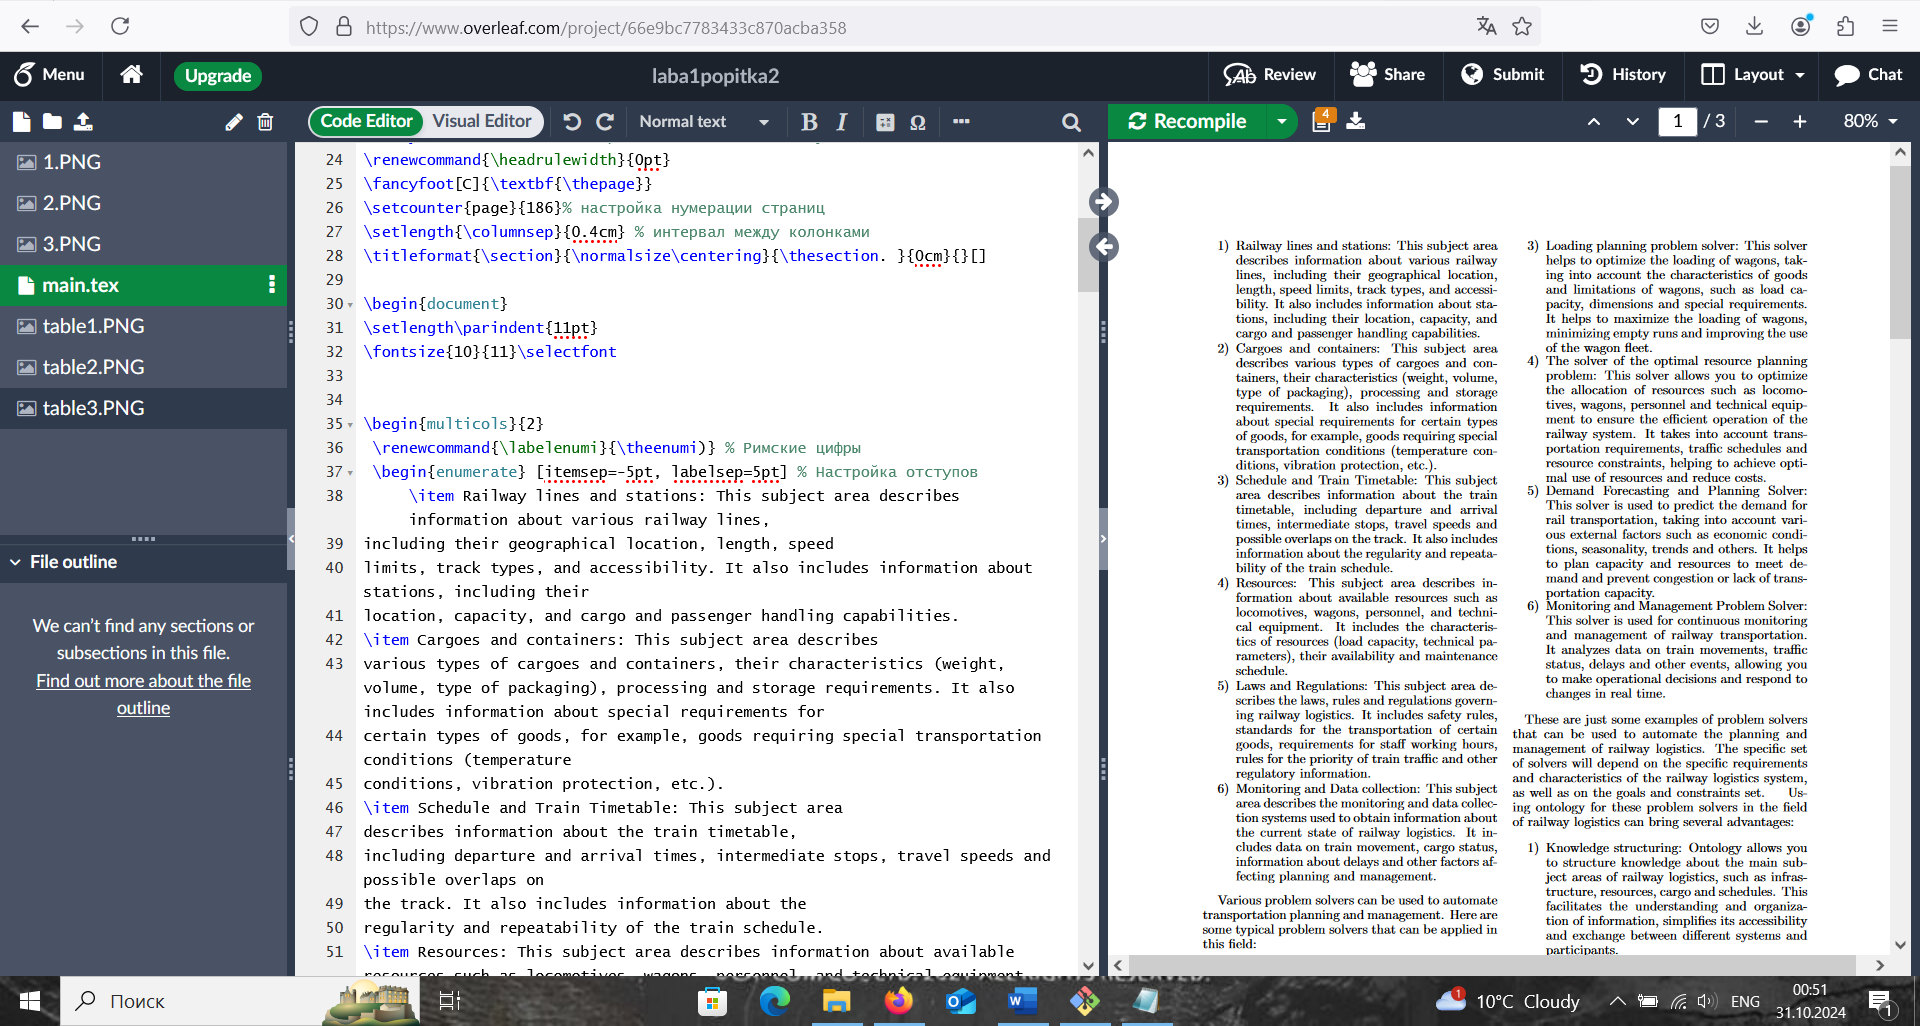
\includegraphics[width=0.48\textwidth]{pic1.png}
    \caption{IDRiD images. From not affected to severe cases}
\end{figure}
\vspace{-0.45cm}
\begin{figure}[H]
    \flushleft
    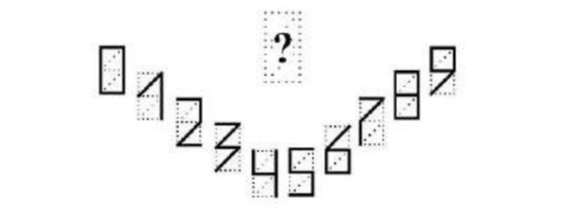
\includegraphics[width=0.48\textwidth]{pic2.png}
    \caption{ACDC MRI image slices}
\end{figure}

\fontsize{10}{14}\selectfont
ACDC dataset contains 150 studies of short-axis car- diac cine MRI of the University Hospital of Dijon patience, 1902 2D slices for training and 1078 2D slices for testing [10]. The 516 photos in the IDRID collection include both pathological and normal retinal fundus [11].
\vspace{0.5cm}

For the purpose of metrics analysis, we sampled a large number of images from each of our trained GANs to see how well it could learn the original data distribution. According to [12], although GANs are characterized by sensitivity to hyperparameters, a subset of GANs are characterized by their oversensitivity, as shown by the sharp change in FID score under different sets of hyperparameters.

Firstly, evaluating set of hyperparameters require some computational time to acxhive best performs for all the GANs described below.
Secondly, GANs are sensitive to the reference dataset: as it increases, image quality improves. To represent difference in GAN characteristics due to dataset size difference all estimation metrics will be evaluated on each dataset with different numbers of training samples.
Each GAN described below produced a batch of two thousand images without additional post processing.

\vspace{0.4cm}
\textit{GAN approaches for realistic data generation}
\vspace{0.2cm}

\textit{1) Deep Convolutions in GAN:} Deep convolutional GANs [13] were one of the first GANs to use con- volutional layers and made significant contributions to balanced GAN learning. Although convolutional layers have been used in GAN architectures before, DCGAN offers an adapted architecture. Several rules have been proposed to create a stable convolutional architecture. Although convolutional networks have been used in GAN architectures before, DCGAN offers an adapted architecture. Several rules have been proposed to create a stable convolutional architecture. These rules are as follows [13]: 
\begin{itemize}[left=1em] % доделать отступы!!!!!
    \item Don’t use merge layers. Instead, use straight line convolutions for the discriminator and fractional line convolutions for the generator.
    \item Use batchnorm in generator and discriminator lay- ers.
\item Do not use fully connected structures in hidden layers.
\item In the output layer of the generator, use the Tanh function, in other layers - the Relu function.
\item Use the LeakyReLU activation function on all dis- criminator layers. 
\end{itemize}
\vspace{0.2cm}

Deep neural networks with a large number of parameters are very powerful machine learning systems. How- ever, a serious problem for such networks is brute force. Large networks are also slow to use, making it difficult to combat overfitting by combining the predictions of many different large neural networks during testing. To solve this problem, the dropout technique is used [14]. Although DCGAN has a variety of advantages over nonconvolutional models, in further chapter we show, that multi-level nonconvolutional GANs outperforms it in terms of the quality of generative image for medical data.

\textit{2) Supervised vs Unsupervised networks:} The variety of image structure is determined by the criteria of realism, which must be described, but at the end of training, such an approach is already meaningless, since the criteria need to be adjusted during the work process. Networks with this approach are called semi-supervised.

In recent years, deep generative models have dramatically pushed forward in generative modelling, achieving state-of-the-art semi-supervised learning results. Unsupervised networks also show good results, but they do not have the same advantages:
\begin{itemize}[left=1em] % доделать отступы!!!!!
 \item The ability to predict H+1 classes (number of classifiers) during training time, forces class labels to be displayed. This extra class correlates with the outputs of generative models and can produce higher quality outputs. This may affect the results of the generative model. We can pass through this class to the corresponding outputs of the generative model, which allows us to improve performance and quality (fewer epochs). This can be compared to the feedback between a discriminator and a generative model.
 \item We can submit softmaxes of fake and original images.
 \item Better pictures and at the same time fewer epochs. 
 \item Possibility of reducing the impact of type I error:
fake images that are perceived as real [15].
The common approaches that have been used in most multi-layer GANs is a progressive growth [16]
\end{itemize}
\textit{3) Progressive growth:} A GAN training methodology that starts with low-resolution images and then gradually increases the resolution by adding layers to the network, as shown in the figure \ref{fig:pic3.png}. This gradual nature of learning allows you to first detect the large-scale structure of the distribution of images (the small size of which, as noted by [16], is characterized by greater stability), and then switch attention to increasingly smaller details, refining and complementing the image, rather than studying all
\end{multicols}
\newpage
\begin{multicols}{2}
\begin{figure}[H]
    \flushleft
    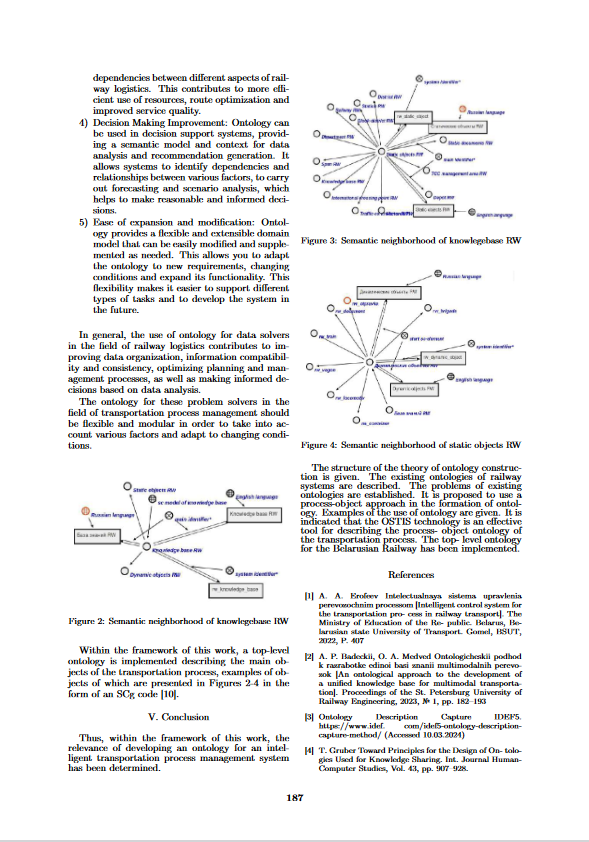
\includegraphics[width=0.48\textwidth]{pic3.png}
    \caption{General architecture of Uncertainty-Guided Progressive GANs
    \label{fig:pic3.png}
}
\end{figure}


\noindent
scales simultaneously. Accordingly, the following advantages can be identified:

\begin{itemize}[left=1em] % доделать отступы!!!!!
\item More stable image generation in the early stages.This is due to less information about classes and fewer modes. The resolution enhancement ap- proach simplifies the task for generating the final images. And this ultimately leads to image stabilization with reliable synthesis of results.
\item Reduced training time.When using progressively growing GANs, most iterations are performed at a lower resolution, and comparable result quality is often achieved 2-6 times faster, depending on the final output resolution.
\item Relatively low GPU requirement [17]. Because GANs at each scale are trained separately, the training process never exceeds a certain maximum size, so GPU requirements remain consistently low, making it easier to generate arbitrarily large images.
\end{itemize}
\vspace{0.1cm}

\textit{4) Multi-scale discriminator:} The [17] used a multi- scale discriminator consisting of two parts of the same structure, which made it possible to solve problems that single-scale discrimination could not handle. The first discriminator, D1, looked at the smaller images to process the overall structure, and the second, D2, helped to reconstruct the finer details of the image. This approach allows you to train a network to find structures in an image more efficiently than single-level GANs. It is also worth noting that this way we can conclude that multi-layer GANs are inherently multi- layer discriminators. In [18], images are generated in several stages (Primary GAN, Subsequent GAN-1, . . . , Subsequent GAN-N) (Figure \ref{fig:pic4.png}).
The output of one phase serves as input to the subsequent GAN in the next phase, explicitly guided by the attention map derived from the uncertainty estimates. Using multi-level generators and discriminators, the authors achieved comprehensive correction of artifacts and noise, potentially replacing additional imaging procedures, which can reduce examination costs and time [18].

A similar approach was used in [19] and [20], where the image was also generated sequentially using enhancement modules (Fig. 6). At the same time, in [21] multi-level generators were used instead of a multilevel discriminator, since it was noted that the instability of the discriminator interferes with focusing on noise removal.
Figure 5. Results of Multi-Scale GANs (MSGANs)
\begin{figure}[H]
    \flushright
    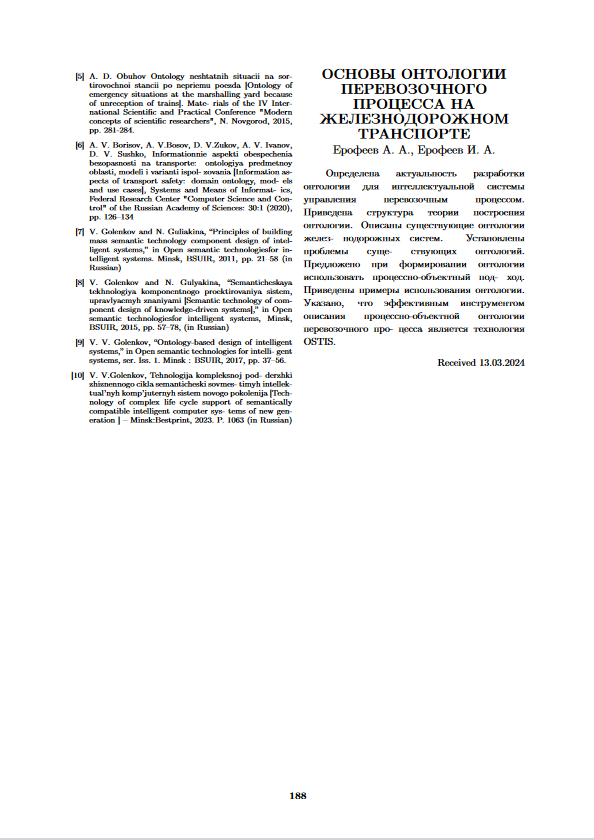
\includegraphics[width=0.48\textwidth]{pic4.png}
    \caption{Results of Multi-Scale GANs (MSGANs)}
    \label{fig:pic4.png}
\end{figure}
\fontsize{10}{14}\selectfont
\noindent
This fact is important, since medical images are susceptible to various noises and artifacts characteristic of different modalities, so it makes sense to consider GAN network architectures where there are no discriminators at certain levels. The [21] architecture is discussed in more detail in a separate paragraph.
\vspace{-0.15cm}
\section{Material and Methods}
\noindent
\textit{A. Modern multi-layer GAN architectures}
\vspace{0.2cm}

Unlike conventional GANs, multi-layer architectures produce higher-quality images. Since, presumably, the discriminator is the largest part responsible for the quality of image synthesis (a similar conclusion can be made based on [22]), in order to avoid errors of the second type. In the case of multi-level GANs, to improve the quality of generation, a load with additional discriminators is used. Also, a significant part of the result depends on the settings of the output layer loss function. In the case of multi-layer GANs, the result of the previous layer goes to the output layer function, which is scaled to the next layer. Thus, such an algorithm is not a multi-level synthesis, but a separation of correct characteristics from incorrect ones. The main advantage of the multi-level GAN architecture is that, unlike single- level ones, it is capable of such separation.
\textit{1) Uncertainty-Guided Progressive GANs (ProGANs):}
In Fig. 4 [18] shows a model consisting of cascaded GANs, where each generator is capable of estimating aleatory uncertainty as well as generating images. This solution removes the above-mentioned limitations of modern methods. Getting rid of them by modeling the underlying distribution of residuals across pixels as an independent but non-identically distributed zero-mean generalized Gaussian distribution (GGD), so
\begin{multline}
    
     \^ b_{ij} = b_{ij} + \epsilon_{ij}\epsilon_{ij} \sim GGD(\epsilon;0,
    \alpha_{ij},\beta_{ij}^{-1}) \equiv \beta_{ij}(2\alpha_{ij} \Gamma(\beta_{ij} ^{-1})^{-1} exp(-\alpha_{ij}^{-1}|\epsilon|^{\beta^{_{ij}}})
\end{multline}

\textit{2) Hierarchical GANs (HierGANs):} HI-GAN [21] consists of four sub-networks, namely Gb, Ga, discriminator Da and boost network $G_c$. Both Gb and Ga genera- tors are DCNNs used for image desaturation. In addition, Ga is trained together with Da to improve its ability to desaturate damaged images and preserve details. The advantage of Ga is its ability to solve the problem of 

\end{multicols}

\end{document}

